\documentclass[aspectratio=169,8pt]{beamer}
\setbeamercolor{frametitle}{fg=black,bg=white}
\setbeamertemplate{frametitle}
{\begin{centering}\smallskip
    \insertframetitle\par
    \smallskip\end{centering}}
\setbeamertemplate{itemize item}{$\bullet$}
\setbeamertemplate{navigation symbols}{}

\setbeamertemplate{navigation symbols}{}
\setbeamertemplate{caption}{\raggedright\insertcaption\par}

\newcommand{\topline}{%
  \begin{tikzpicture}[remember picture,overlay]
   \node[xshift=0.5\paperwidth,yshift=-1cm] at (current page.north west){%
    
\includegraphics[width=\paperwidth]{i/line.png}};
  \end{tikzpicture}
}

\long\def\bframe#1#2\eframe{\begin{frame}{#1}\topline#2\end{frame}}
\long\def\bbframe#1\eframe{\begin{frame}#1\end{frame}}
\long\def\be#1\ee{\begin{align*}#1\end{align*}}
\long\def\bcc#1\ecc{\begin{columns}#1\end{columns}}
\long\def\bc#1\ec{\begin{column}{0.48\textwidth}#1\end{column}}
\newcommand{\fig}[1]{%
  \begin{center}
    \includegraphics[width=\textwidth]{#1}
\end{center}}
\newcommand{\wfig}[2]{%
  \begin{center}
    \includegraphics[width=#1\textwidth]{#2}
  \end{center}}
\newcommand{\ffig}[2]{%
    \includegraphics[width=#1\textwidth]{#2}}

\usepackage{tikz}
\usepackage{helvet}
%\usepackage[export]{adjustbox}
%\usepackage{makecell}


\begin{document}

\bframe{Shallow analogy with biological neural networks}
Discussion about biological NN is not connected to the proposed model.
\eframe

\bframe{Evolvable Neural Units (ENU) is butchered GRU}
\begin{center}
  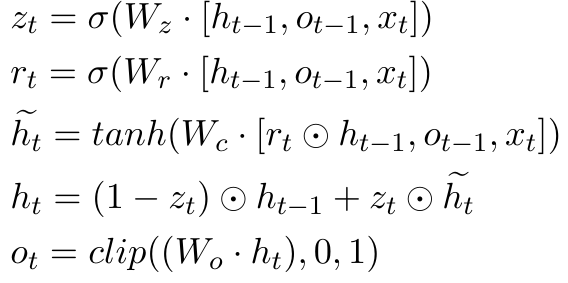
\includegraphics[width=0.50\textwidth]{i/eq.png}
\end{center}
ENU is GRU with output plugged into internals \\
No motivation for the change is given \\
``Evolvable'' means un-trainable: suffers from vanishing gradient problem
\eframe

\bframe{Spiking Neurons}

Current GPUs, however, are little ovens, much
hungrier for energy than biological brains.
...
In practical applications, however,current artificial networks of
spiking neurons cannot yet compete withth best traditional NN
(J. Schmidhuber, 2015)

\begin{center}
  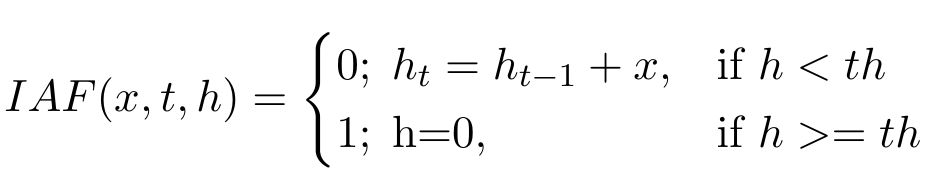
\includegraphics[width=0.80\textwidth]{i/iaf.png}
\end{center}
\eframe

\bframe{STDP}

``Spike Timing Dependent Plasticity (STDP) is a temporally asymmetric
form of Hebbian learning induced by tight temporal correlations
between the spikes of pre- and postsynaptic neurons. As with other
forms of synaptic plasticity, it is widely believed that it underlies
learning and information storage in the brain.''
\\
``A paradox in auditory and electrosensory neural systems is that they
encode behaviourally relevant signals in the range of a few
microseconds with neurons that are at least one order of magnitude
slower. A central question is whether neuronal firing can be more
precise than the time constants of the neuronal processes involved.''

\eframe

\bframe{Meaningless comparison}
\begin{center}
  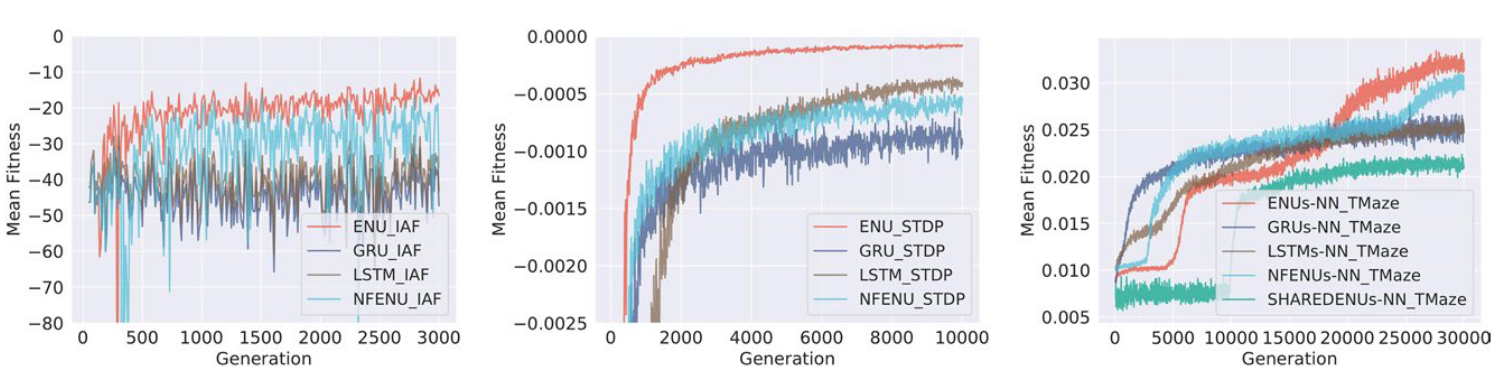
\includegraphics[width=0.90\textwidth]{i/lines.png}
\end{center}
random search path depends on initial condition \\
backproparation is a supperior way to train GRU and LSTM
\eframe

\bframe{Crippled artificial life toy is an example of meta-learning?}
\begin{center}
  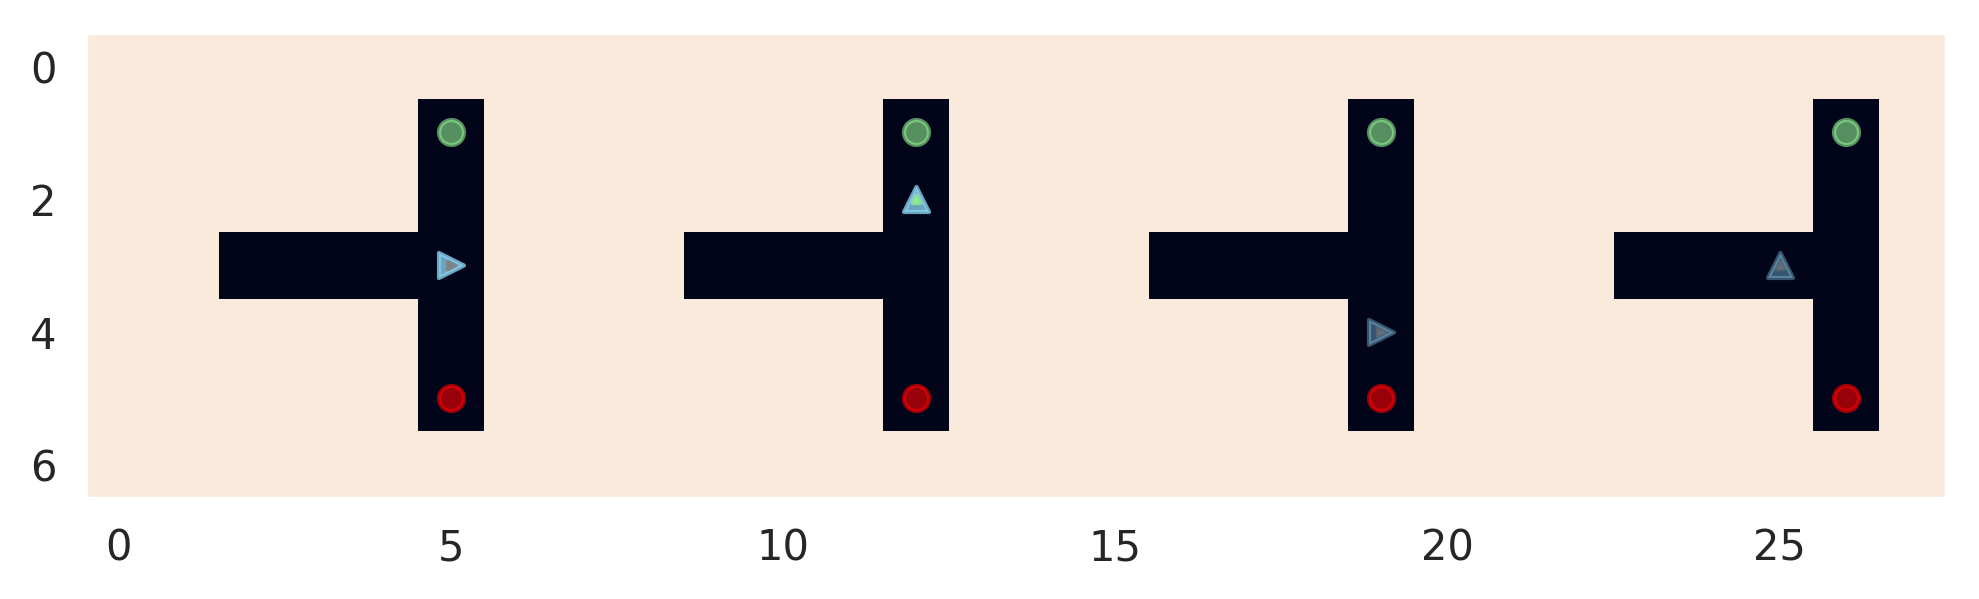
\includegraphics[width=0.75\textwidth]{i/maze.png}
\end{center}
The state is very small (5x4): position, orientation, flag if food was seen. \\
Can be solved by a tabular method
\eframe

\end{document}
